
% Титульный слайд
\begin{frame}[noframenumbering, plain]
    \setcounter{framenumber}{1}
    \maketitle
\end{frame}

\section{Введение}

\begin{frame}{Постановка задачи}
	\textbf{\underline{Цель диссертационной работы}}: разработка методики коррекции расчетных моделей летательных аппаратов по результатам модальных испытаний.
	\begin{center}
		\includegraphics[width = 0.6\textwidth]{large-reflector}
	\end{center}
\end{frame}

\begin{frame}{Алгоритм решения проблемы}
	\begin{columns}
		\begin{column}{0.5\textwidth}
			\centering
			\fbox{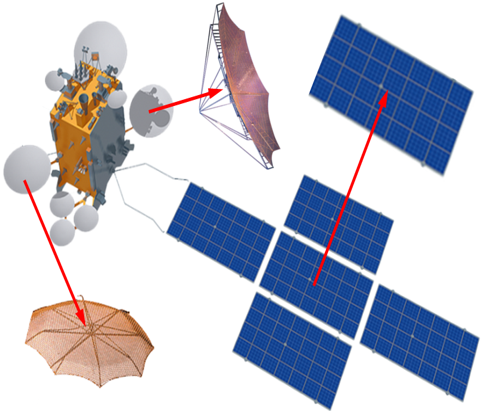
\includegraphics[width=1\textwidth]{decomposition}}
		\end{column}
		\begin{column}{0.5\textwidth}
			\centering
			% Определение стиля
			\tikzstyle{blockWide}=[rectangle, draw = black, fill = blue!20, rounded corners, text width = 20em, text centered, minimum height = 1.5em, drop shadow] % Блок
			\tikzstyle{blockWideC}=[blockWide, fill = red!20]
			\tikzstyle{arrow} = [draw, thick, color=black!90, -latex'] % Стрелка
			\scriptsize % Размер шрифта
			% Задание перменных
			\def\nodeDist{0.3cm} % Дистанция между узлами
			% Отрисовка блок-схемы
			\begin{tikzpicture}[scale = 1, transform shape]
				% Задание узлов		
				\node (modalTests) [blockWide] {Модальные испытания составных частей конструкции};
				\node (modelUpdating) [blockWide, below = \nodeDist of modalTests] {Коррекция расчетных моделей составных частей конструкции по результатам испытаний};
				\node (checkInfluence) [blockWide, below = \nodeDist of modelUpdating] {Освобождение закрепленных расчетных моделей составных частей конструкции};
				\node (buildRealModel) [blockWide, below = \nodeDist of checkInfluence] {Синтез расчетной модели полной конструкции из её составных частей};
				\node (buildMathModel) [blockWide, below = \nodeDist of buildRealModel] {Определение динамических характеристик полной расчетной модели};
				% Соединение узлов
				\draw [arrow] (modalTests.south) -- (modelUpdating.north);
				\draw [arrow] (modelUpdating.south) -- (checkInfluence.north);
				\draw [arrow] (checkInfluence.south) -- (buildRealModel.north);
				\draw [arrow] (buildRealModel.south) -- (buildMathModel.north);
			\end{tikzpicture}
		\end{column}
	\end{columns}
\end{frame}

\begin{frame}{Задачи исследования}
	\begin{enumerate}
		\item Разработать методику коррекции расчетных динамических моделей ЛА по экспериментально определенным модальным характеристикам.
		\item Изучить методы классического модального анализа. Создать комплекс программ для обработки и представления результатов модального анализа непосредственно в процессе испытаний.
		\item Изучить методы операционного модального анализа. Разработать программное обеспечение для определения модальных характеристик ЛА по результатам акустических и летных испытаний.
		\item Изучить методы вибродиагностики конструкций. Разработать программное обеспечение для контроля конструктивно-производственных дефектов в конструкциях ЛА в процессе модальных испытаний.
		\item Оценить сходимость и чувствительность методики коррекции к погрешностям в результатах модальных испытаний.
		\item Решить практические задачи коррекции расчетных моделей конструкций.
	\end{enumerate}
\end{frame}

\begin{frame}{Положения, выносимые на защиту}
	\begin{enumerate}
		\item Методика коррекции расчетных динамических моделей путем добавления корректирующих конечных элементов, параметры которых определяются из решения задачи оптимизации по целевым модальным характеристикам.
		\item Методика синтеза расчетной модели ЛА из полноразмерных моделей составных частей, скорректированных по результатам модальных испытаний.
		\item Комплекс программ для обработки и представления результатов экспериментального модального анализа. Программное обеспечение коррекции и синтеза расчетных моделей ЛА.
		\item Результаты исследования сходимости алгоритма и чувствительности методики коррекции расчетных моделей к погрешностям эксперимента.
		\item Результаты решения практических задач.
	\end{enumerate}
\end{frame}

\section{Методика коррекции динамических свойств КЭ-модели}

\begin{frame}{Методика коррекции конечно-элементной модели}
	\begin{block}{Обобщенная проблема собственных значений}
		\begin{equation}
			(\mat{K} - \lambda \mat{M}) \mat{Y} = 0,
		\end{equation}
		где $ \mat{K} $, $ \mat{M} \in \set{R} ^ {n \times n}$~---~матрицы жесткости и масс; $ \mat{Y} $~---~формы собственных колебаний; $ \lambda $~---~собственные числа; $ N $~---~число степеней свободы.
	\end{block}
	\begin{block}{Корректирующая матрица жесткости в общем виде}
 		\begin{equation}
 			\begin{gathered}
 				\Delta \mat{K} = \Delta \internal{\mat{K}} + \Delta \external{\mat{K}}, \\
				\Delta \internal{\mat{K}}_j = \sum\limits_{p\,=\,1}^{q} \internal{c}_{j+p-1} \mat{G}_j^{(p)}, \ j = 1 \hdots e, \\
				\Delta \external{\mat{K}} = \operatorname{diag} \cbrackets{\external{c}_1, \external{c}_2, \hdots, \external{c}_N}.
			\end{gathered}
		\end{equation}
		где $ \internal{\mat{c}} $ и $ \external{\mat{c}} $~---~внутренние и внешние корректирующие жесткости; $ q $~---~число внутренних парциальных корректирующих жесткостей, описывающих элемент; $ \mat{G}_j^{(p)} $~---~парциальная матрица жесткости внутреннего коррректирующего элемента; $ e $~---~число внутренних корректирующих элементов.
	\end{block}
\end{frame}

\begin{frame}{Внутренний корректирующий элемент в виде балки}
	\begin{block}{Парциальные корректирующие матрицы жесткости}
		\begin{equation*}
		\begingroup
		\setlength\arraycolsep{2pt}
		\begin{gathered}
			\mat{G}_j^{(1)} =
			\begin{pmatrix}
				\mat{D}_1 & \mat{0} & -\mat{D}_1 & \mat{0} \\
				\mat{0} & \mat{0} & \mat{0} & \mat{0} \\
				-\mat{D}_1 & \mat{0} & \mat{D}_1 & \mat{0} \\
				\mat{0} & \mat{0} & \mat{0} & \mat{0} \\
			\end{pmatrix},
			\mat{G}_j^{(2)} =
			\begin{pmatrix}
				6 \mat{D}_2 & 3 \ell \mat{D}_4 & -6 \mat{D}_2 & 3 \ell \mat{D}_4 \\
				3 \ell \trans{\mat{D}}_4 & 2 \ell ^ 2 \mat{D}_3 & -3 \ell \trans{\mat{D}}_4 & \ell ^ 2 \mat{D}_3 \\
				-6 \trans{\mat{D}}_2 & -3 \ell \mat{D}_4 & 6 \mat{D}_2 & -3 \ell \mat{D}_4 \\
				3 \ell \trans{\mat{D}}_4 & \ell ^ 2 \trans{\mat{D}}_3 & -3 \ell \trans{\mat{D}}_4 & 2 \ell ^ 2 	\mat{D}_3
			\end{pmatrix}, \\
			\mat{G}_j^{(3)} =
			\begin{pmatrix}
				6 \mat{D}_3 & -3 \ell \trans{\mat{D}}_4 & -6 \mat{D}_3 & -3 \ell \trans{\mat{D}}_4 \\
				-3 \ell \mat{D}_4 & 2 \ell ^ 2 \mat{D}_2 & 3 \ell \mat{D}_4 & \ell ^ 2 \mat{D}_2 \\
				-6 \trans{\mat{D}}_3 & 3 \ell \trans{\mat{D}}_4 & 6 \mat{D}_3 & 3 \ell \trans{\mat{D}}_4 \\
				-3 \ell \mat{D}_4 & \ell ^ 2 \trans{\mat{D}}_2 & 3 \ell \mat{D}_4 & 2 \ell ^ 2 \mat{D}_2
			\end{pmatrix},
			\mat{G}_j^{(4)} =
			\begin{pmatrix}
				\mat{0} & \mat{0} & \mat{0} & \mat{0} \\
				\mat{0} & \mat{D}_1 & 0 & -\mat{D}_1 \\
				\mat{0} & \mat{0} & \mat{0} & \mat{0} \\
				\mat{0} & -\mat{D}_1 & 0 & \mat{D}_1 \\
			\end{pmatrix},
		\end{gathered}
		\endgroup
		\end{equation*}
	\end{block}
	\begin{block}{Матрицы из направляющих косинусов}
		\begin{equation*}
			\mat{D}_k = 
			\begin{pmatrix}
				d_{k, 1}^2 & d_{k, 1} d_{k, 2} & d_{k, 1} d_{k, 3} \\
				d_{k, 2} d_{k, 1} & d_{k, 2} ^ 2 & d_{k, 2} d_{k, 3} \\
				d_{k, 3} d_{k, 1} & d_{k, 3} d_{k, 2} & d_{k, 3} ^ 2
				\end{pmatrix},
			\mat{D}_4 = 
			\begin{pmatrix}
				d_{2, 1} d_{3, 1} & d_{2, 1} d_{3, 2} & d_{2, 1} d_{3, 3} \\
				d_{2, 2} d_{3, 1} & d_{2, 2} d_{3, 2} & d_{2, 2} d_{3, 3} \\
				d_{2, 3} d_{3, 1} & d_{2, 3} d_{3, 2} & d_{2, 3} d_{3, 3}
			\end{pmatrix},
		\end{equation*}
	\end{block}
	где $ \ell $~---~длина корректирующего балочного элемента, $ k = 1 \hdots 3 $.
\end{frame}

\begin{frame}{Принципиальная схема коррекции}
	\centering
	\begin{tikzpicture}[scale = 1]
		\pgfmathsetmacro{\nodeDist}{0.1}
		\pgfmathsetmacro{\shiftText}{0.0}
		% Исходная модель
		\node[inner sep = 0pt] (initial) at (0, 0) {\includegraphics[width = 0.4\textwidth]{simple-model-initial}};
		\node[inner sep = 0pt, below = \shiftText of initial.south] (textInitial) {Исходная модель};
		% Знак
		\node [below = \nodeDist of textInitial.south, color = blue] (sumSign) {\huge \bfseries +};
		% Коррректирующие элементы
		\node[inner sep = 0pt, below = -\nodeDist of sumSign.south] (elements) {\includegraphics[width = 0.4\textwidth]{simple-model-elements}};
		\node[inner sep = 0pt, below = \shiftText of elements.south] (textElements) {Корректирующие элементы};
		% Скорректированная модель
		\draw [-{Latex[length = 4mm]}, color = red, very thick](sumSign.east) ++ (2, 0) --++ (1, 0) node [right] (updated) {\includegraphics[width = 0.5\textwidth]{simple-model-updated}};
		\node[inner sep = 0pt, below = \shiftText of updated.south] (textUpdated) {Скорректированная модель};
	\end{tikzpicture}
\end{frame}

\begin{frame}{Расчет корректирующих жесткостей}
	\begin{block}{Задача безусловной минимизации}
		\vspace{-1em}
		\begin{gather}
			f_j(c) = \mat{Y}_j^{(0)\mathsf{T}} \Delta \mat{K}^{(i+1)} \mat{Y}_j^{(i)} + \mat{Y}_j^{(0)\mathsf{T}} \mat{K} \Delta \mat{Y}_j^{(i)} - \Delta \lambda^*_j, \\
			F(c) = \sum \limits_{j\,=\,1}^s w_i f_j^2(c) + w_c \sum \limits_{k\,=\,1}^m c_k^2 \rightarrow \min_{c},
		\end{gather}
		где $ i $~---~номер текущей итерации, $ \Delta \lambda^*_j = \lambda_j^* - \lambda_{j0} $ ($\lambda_j^*$~---~целевые собственные значения), $ w_i $~---~весовые коэффициенты, $ s $~---~число целевых частот, $ w_c $~---~параметр регуляризации.
	\end{block}	
	\begin{block}{Нормировка собственных векторов}
		\vspace{-1em}
		\begin{gather}
			\mat{Y}^{(0)\mathsf{T}} \mat{M} \mat{Y}^{(0)} = 1, \\
			\mat{Y}^{(0)\mathsf{T}} \mat{M} \mat{Y}^{(i)} = 1 \Longrightarrow \mat{Y}^{(0)T} \mat{M} \Delta \mat{Y}^{(i)} = 0,
		\end{gather}
		где $ \mat{Y}^{(0)} $, $ \mat{Y}^{(i)} $~---~исходные и текущие собственные вектора.
	\end{block}	
\end{frame}

\begin{frame}{Формирование матрицы демпфирования в физической системе координат}
	\begin{block}{Нулевое приближение (гипотеза Е.\,C.~Сорокина)}
		\begin{gather}
			\mat{H} = \alpha \tilde{\mat{K}} + \beta \mat{M}, \\
			G(\alpha, \beta) = \sum\limits_{i\,=\,1}^p w_i \left( 1 - \frac{\alpha \tilde{\kappa}_i + \beta \mu_i}{h_i} \right)^2 \rightarrow \min_{\alpha, \beta},
		\end{gather}
		где $ \alpha $ и $ \beta $~---~коэффициенты конструкционного и инерционного демпфирования, $ h $~---~целевые обобщенные коэффициенты демпфирования, $ p $~---~число целевых коэффициентов.
	\end{block}
	\begin{block}{Преобразование матрицы демпфирования} 
 		\begin{equation} 
			\tilde{\mat{H}} = \mat{H} + \Delta \internal{\mat{H}} + \Delta \external{\mat{H}},
		\end{equation}
		где $ \Delta \internal{\mat{H}} $ и $ \Delta \external{\mat{H}} $~---~матрицы демпфирования внутренних и внешних корректирующих элементов. 
	\end{block}
\end{frame}

\begin{frame}{Методика освобождения КЭ-модели от закреплений}
	\begin{equation} 
		\begin{pmatrix}
			\mat{K} & -(\sum k)^\intercal \\
			 -\sum k & \mat{0} 
		\end{pmatrix} 
		\begin{Bmatrix}
			\tilde{X} \\ 
			\xi
		\end{Bmatrix}			
		+ 
		\begin{pmatrix}
			\mat{M} & \mat{0} \\
			\mat{0} & \mu - \sum \sum m
		\end{pmatrix}
			\begin{Bmatrix}
			\ddot{\tilde{\mat{X}}} \\ 
			\ddot{\mat{\xi}}
		\end{Bmatrix}	
		= 0,
	\end{equation}
	\begin{itemize}
		\item $ \mat{K}, \mat{M} \in R ^ {n \times n} $~---~матрицы жесткости и масс закрепленной модели,
		\item $ \mu \in R^{6 \times 6} $~---~матрица инерции,
		\item $ \xi $~---~вектор перемещений как жесткого целого,
		\item $ \tilde{\mat{X}} $~---~вектор перемещений свободной модели,
		\item $ \sum k = F_s(\mat{K}) \in R ^ {6 \times n}$, $ \sum \sum m = F_m(F_s(\mat{M})) \in R ^ {6 \times 6} $~{\footnotemark}.
	\end{itemize}
	\vfill
	\footnotetext[1]{Матричные функции $ F_s,\ F_m $ представлены на следующем слайде.}
\end{frame}

\begin{frame}{Матричные функции $ F_m $ и $ F_s $}
	\begingroup
	\setlength\arraycolsep{2pt}
	\begin{gather*}
		\small
		F_m(\mat{A})
		= \left(
		\begin{matrix}
			\sum \limits_{i=1}^N a_{1,G_{i,1}} 
			& \hdots
			& \sum \limits_{i=1}^N a_{1,G_{i,3}} 
			&
			\sum\limits_{i=1}^N
			\left(
			\begin{matrix}
				a_{1,G_{i,4}} + \\
				+ \Delta y_i^0 a_{1, G_{i,3}} - \\
				- \Delta z_i^0 a_{1, G_{i,2}} \\
			\end{matrix} \right)
			& 
			\hdots
			&
			\sum\limits_{i=1}^N
			\left(
			\begin{matrix}
				a_{1,G_{i,6}} + \\
				+ \Delta x_i^0 a_{1, G_{i,2}} - \\
				- \Delta y_i^0 a_{1, G_{i,1}} \\
			\end{matrix} \right) \\ 
			\hdots & \hdots & \hdots & \hdots & \hdots & \hdots \\
			\sum \limits_{i=1}^N a_{6,G_{i,1}} 
			& \hdots 
			& \sum \limits_{i=1}^N a_{6,G_{i,3}} 
			&
			\sum\limits_{i=1}^N
			\left(
			\begin{matrix}
				a_{6,G_{i,4}} + \\
				+ \Delta y_i^0 a_{6, G_{i,3}} - \\
				- \Delta z_i^0 a_{6, G_{i,2}} \\
			\end{matrix} \right)
			& 
			\hdots
			&
			\sum\limits_{i=1}^N
			\left(
			\begin{matrix}
				a_{6,G_{i,6}} + \\
				+ \Delta x_i^0 a_{6, G_{i,2}} - \\
				- \Delta y_i^0 a_{6, G_{i,1}} \\
			\end{matrix} \right) \\ 
		\end{matrix}
		\right), \\ 
		\small
		F_s(\mat{A}) ^ \intercal
		= \left(
		\begin{matrix}	
			\sum \limits_{i=1}^N a_{G_{i,1}, 1} 
			& \hdots 
			& \sum \limits_{i=1}^N a_{G_{i,3}, 1} 
			&
			\sum\limits_{i=1}^N
			\left(
			\begin{matrix}
				a_{G_{i,4}, 1} + \\
				+ \Delta y_i^0 a_{G_{i,3}, 1} - \\
				- \Delta z_i^0 a_{G_{i,2}, 1} \\
			\end{matrix} \right)
			& 
			\hdots
			&
			\sum\limits_{i=1}^N
			\left(
			\begin{matrix}
				a_{G_{i,6}, 1} + \\
				+ \Delta x_i^0 a_{G_{i,2}, 1} - \\
				- \Delta y_i^0 a_{G_{i,1}, 1} \\
			\end{matrix} \right) \\ 
			\hdots & \hdots & \hdots & \hdots & \hdots & \hdots \\
			\sum \limits_{i=1}^N a_{G_{i,1},n} 
			& \hdots
			& \sum \limits_{i=1}^N a_{G_{i,3},n} 
			&
			\sum\limits_{i=1}^N
			\left(
			\begin{matrix}
				a_{G_{i,4},n} + \\
				+ \Delta y_i^0 a_{G_{i,3}, n} - \\
				- \Delta z_i^0 a_{G_{i,2}, n} \\
			\end{matrix} \right)	
			& 
			\hdots
			&
			\sum\limits_{i=1}^N
			\left(
			\begin{matrix}
				a_{G_{i,6}, n} + \\
				+ \Delta x_i^0 a_{G_{i,2}, n} - \\
				- \Delta y_i^0 a_{G_{i,1}, n} \\
			\end{matrix} \right) \\ 
		\end{matrix}
		\right),
	\end{gather*}
	\endgroup
	где $ G_{i, j} $~---~номер уравнения $ i $-го узла $ j $-ой степени свободы; $ a_{i,j}$~---~элементы матрицы $ \mat{A} $; $ \Delta x^0_i, \Delta y^0_i, \Delta z^0_i $~---~компоненты радиус-вектора от центра тяжести до $ i $-го узла недеформированной конструкции.
\end{frame}

\section{Оценка чувствительности методики коррекции}

\begin{frame}{Оценка чувствительности методики коррекции}
	\textbf{\underline{Цель}}: оценка влияния погрешностей в экспериментальном определении частот на устойчивость результата коррекции. \\
	\textbf{\underline{Алгоритм}}
	\begin{enumerate}
		\item Вычисление частот и форм собственных колебаний исходной модели.
		\item Варьирование числа корректируемых тонов собственных колебаний и внесение случайных отклонений $ \Delta \mat{f} \sim \set{N} \rbrackets{\mu, \sigma ^ 2} $ в значения частот. 
		\item Решение задачи коррекции. Определение максимальной погрешности критерия модального соответствия $ \varepsilon_{\mathrm{MAC}} $ между исходными и полученными формами колебаний.
		\item Оценка первого центрального момента $ \mu_1\rbrackets{\varepsilon_{\mathrm{MAC}}} $ в зависимости от числа независимых испытаний с целью получения достоверных оценок математического ожидания и дисперсии. 
		\item Последовательность шагов 2~--~4 повторяется до тех пор, пока $ \mu_1\rbrackets{\varepsilon_{\mathrm{MAC}}} $, рассчитанный для выборки из последних наблюдений, не стабилизируется с заданной точностью.
	\end{enumerate}
\end{frame}

\begin{frame}{Оценка чувствительности методики коррекции}
	\textbf{\underline{Цель}}: оценка влияния погрешностей в экспериментальном определении частот на устойчивость результата коррекции. \\
	\textbf{\underline{Алгоритм}}
	\begin{enumerate}
		\item Вычисление частот и форм собственных колебаний исходной модели.
		\item Варьирование числа корректируемых тонов собственных колебаний и внесение случайных отклонений $ \Delta \mat{f} \sim \set{N} \rbrackets{\mu, \sigma ^ 2} $ в значения частот. 
		\item Решение задачи коррекции. Определение максимальной погрешности критерия модального соответствия $ \varepsilon_{\mathrm{MAC}} $ между исходными и полученными формами колебаний.
		\item Оценка первого центрального момента $ \mu_1\rbrackets{\varepsilon_{\mathrm{MAC}}} $ в зависимости от числа независимых испытаний с целью получения достоверных оценок математического ожидания и дисперсии. 
		\item Последовательность шагов 2~--~4 повторяется до тех пор, пока $ \mu_1\rbrackets{\varepsilon_{\mathrm{MAC}}} $, рассчитанный для выборки из последних наблюдений, не стабилизируется с заданной точностью.
	\end{enumerate}
\end{frame}

\begin{frame}{Оценка чувствительности на примере свободной прямоугольной пластины}
	\begin{center}	
		\begin{columns}
			\begin{column}{0.5\textwidth}
				\centering
				\begin{figure}
					\includegraphics[width = 1\textwidth]{perturbation-plate-convergence}
					\caption{Погрешность определения форм колебаний в зависимости от погрешности целевых частот}
				\end{figure}
			\end{column}
			\begin{column}{0.5\textwidth}
				\centering
				\vspace{-0.9em}
				\begin{figure}
					\includegraphics[width = 1\textwidth]{perturbation-plate-samplesize}
					\caption{Число независимых испытаний в зависимости от погрешности целевых частот}
				\end{figure}
			\end{column}
		\end{columns}
	\end{center}
\end{frame}

\begin{frame}{Тестирование методики синтеза на расчетной модели космического аппарата (КА)}
	\begin{figure}
		\centering
		\includegraphics[width = 1\textwidth]{spacecraft-test-mesh}
	\end{figure}
	Число степеней свободы: $ 18714 $.
\end{frame}

\begin{frame}{Коррекция моделей составных частей тестового КА}
	\begin{figure}
		\centering
		\begin{subfigure}[t]{0.45\textwidth}
			\centering
			\includegraphics[width = \textwidth]{test-spacecraft-orbital-distribution}
			\caption{Орбитальный модуль} 
		\end{subfigure}
		\hfill
		\begin{subfigure}[t]{0.45\textwidth}
			\centering
			\includegraphics[height = \textwidth]{test-spacecraft-panel-distribution}
			\caption{Панели солнечных батарей} 
		\end{subfigure} 
		\caption{Изменения узловых жесткостей при коррекции составных частей}
	\end{figure}	
\end{frame}

\begin{frame}{Результаты синтеза глобальной модели КА}
	\begin{tblr}{
		colspec = {|X[c, -1]|X[c]|X[c]|X[c]|X[c]|},
		width = \textwidth, 
		hlines
	}
		\SetCell[r = 3]{c} № тона & \SetCell[c = 4]{c} Погрешность в частотах собственных колебаний, \% &&& \\
		& \SetCell[r = 2]{c} Без коррекции & \SetCell[c = 3]{c} Коррекция по девяти частотам && \\
		& & Панелей & Модуля & Панелей и модуля \\ \hline
		7 & -4.689 & -2.120 & -2.756 & -0.021 \\
		8 & -4.678 & -2.078 & -2.782 & -0.018 \\
		9 & -5.121 & -4.447 & -0.674 & 0.100  \\
		10 & -5.040 & -4.760 & -0.354 & -0.028 \\
		11 & -5.040 & -4.760 & -0.357 & -0.032 \\
		12 & -5.121 & -4.443 & -0.687 & 0.091 \\
		13 & -4.102 & -0.966 & -3.161 & 0.011 \\
		14 & -4.112 & -0.999 & -3.135 & 0.016 \\
		15 & -3.303 & -0.234 & -3.066 & -0.006 \\
	\end{tblr}
\end{frame}